\documentclass[11pt]{article}
\usepackage[margin=1in]{geometry}
\usepackage[T1]{fontenc}
\usepackage{amsmath,amssymb,amsthm,booktabs,array,longtable}
\usepackage{graphicx}
\usepackage{float}
\usepackage[hidelinks]{hyperref}
\usepackage{enumitem}
\graphicspath{{figures/}}

\title{DS5020 Final Project -- Iterations 2 and 3\\[3pt]\large Bayesian A/B Testing: Mathematical Foundations, Implementation, and Verification}
\author{Kamya Kanara \and Rishita Chawla \and Vaibhavi}
\date{Fall 2026}

\newtheorem{proposition}{Proposition}
\newtheorem{definition}{Definition}
\newcommand{\signoff}[2]{\par\smallskip\noindent\textit{Owner: #1\quad Checked by: #2}\par}
\newcommand{\E}{\mathbb{E}}
\newcommand{\Var}{\operatorname{Var}}
\newcommand{\Beta}{\operatorname{Beta}}

\begin{document}
\maketitle
\begin{abstract}
This report develops the mathematical foundation for Bayesian A/B testing and documents a from-scratch numerical implementation and independent verification in Iteration 3. We model a binary outcome in each group with a Binomial likelihood and a Beta prior, derive the Beta posterior and its moments, derive a Monte Carlo estimator for $P(p_B>p_A\mid\text{data})$ together with its standard error, and derive the pooled two-proportion $z$-test as a frequentist comparison. A known-truth simulation checks every derivation numerically, and the Cookie Cats randomized experiment is described as the real dataset. In the real data, \texttt{gate\_30} has higher observed retention than \texttt{gate\_40} for both day-one and day-seven outcomes; the day-seven difference is clear in both the Bayesian and frequentist analyses, while the day-one difference is not significant at the 5\% level.
\end{abstract}

\section{Project objective and scope}
The objective is to compare the success probabilities of two versions, A and B, and to quantify uncertainty about which version performs better. For the Cookie Cats application, one trial is one player, the two groups are the assigned game versions (\texttt{gate\_30} $=$ A and \texttt{gate\_40} $=$ B), and a ``success'' (the analogue of a click) is a player returning to the game. Day-one retention is the primary outcome and day-seven retention is a secondary outcome.

\section{Notation}
\begin{longtable}{l p{0.72\textwidth}}
\toprule
\textbf{Symbol} & \textbf{Meaning / dimension}\\
\midrule
\endhead
$g\in\{A,B\}$ & Group index.\\
$n_A,n_B$ & Number of independent trials in groups A and B; positive integers.\\
$x_A,x_B$ & Number of successes in groups A and B; integers with $0\le x_g\le n_g$.\\
$Y_{g,i}$ & Outcome of trial $i$ in group $g$; $Y_{g,i}\in\{0,1\}$.\\
$p_A,p_B$ & Unknown success probabilities; scalars in $[0,1]$.\\
$\hat p_A,\hat p_B$ & Observed proportions $x_A/n_A$, $x_B/n_B$; scalars.\\
$a,b$ & Beta prior shape parameters, $a,b>0$; scalars.\\
$\alpha_g,\beta_g$ & Posterior Beta shape parameters, $\alpha_g=a+x_g$, $\beta_g=b+n_g-x_g$; scalars.\\
$s_g$ & $\alpha_g+\beta_g=a+b+n_g$.\\
$M$ & Number of Monte Carlo posterior draws; positive integer.\\
$p_A^{(m)},p_B^{(m)}$ & $m$-th posterior draw for each group, $m=1,\dots,M$.\\
$I_m$ & Indicator $\mathbb 1\{p_B^{(m)}>p_A^{(m)}\}\in\{0,1\}$.\\
$q$ & The posterior probability $P(p_B>p_A\mid\text{data})\in[0,1]$.\\
$\hat q$ & Monte Carlo estimate of $q$.\\
$\mu_0$ & Prior mean $a/(a+b)$ for the Beta prior.\\
$w$ & Data weight $n/(a+b+n)$ in the posterior-mean weighted average.\\
$\alpha_{\mathrm{sig}}$ & Chosen significance level for a frequentist hypothesis test (here, $0.05$).\\
$\hat p_{\mathrm{pool}}$ & Pooled proportion $(x_A+x_B)/(n_A+n_B)$.\\
$SE_0$ & Null standard error of $\hat p_B-\hat p_A$.\\
$z$ & Standardized test statistic; $\Phi$ is the standard normal CDF.\\
\bottomrule
\end{longtable}
All quantities in this project are scalars ($1\times1$); there are no matrices. Data are stored as two length-$n_g$ binary vectors $Y_g\in\{0,1\}^{n_g}$.

\section{Definitions}
\begin{definition}[Bernoulli trial]
A Bernoulli trial has outcome $Y\in\{0,1\}$ with $P(Y=1)=p$ and $P(Y=0)=1-p$.
\end{definition}
\begin{definition}[Binomial distribution]
If $X$ counts successes in $n$ independent Bernoulli trials with common success probability $p$, then
$P(X=x\mid n,p)=\binom{n}{x}p^x(1-p)^{n-x}$, $x=0,\dots,n$.
\end{definition}
\begin{definition}[Beta function and Beta distribution]
For $a,b>0$ the beta function is $B(a,b)=\int_0^1u^{a-1}(1-u)^{b-1}\,du=\Gamma(a)\Gamma(b)/\Gamma(a+b)$, where $\Gamma(t+1)=t\,\Gamma(t)$. A random variable $p$ has a $\Beta(a,b)$ distribution if it has density $f(p\mid a,b)=p^{a-1}(1-p)^{b-1}/B(a,b)$ on $0<p<1$.
\end{definition}
\begin{definition}[Conditional probability and Bayes' theorem]
$P(A\mid B)=P(A\cap B)/P(B)$ for $P(B)>0$. For a parameter $p$ and data $x$, Bayes' theorem gives $\pi(p\mid x)=P(x\mid p)\pi(p)/P(x)$, so $\pi(p\mid x)\propto P(x\mid p)\pi(p)$ as a function of $p$.
\end{definition}
\begin{definition}[Prior, likelihood, posterior]
The prior $\pi(p)$ describes $p$ before seeing data; the likelihood is $P(x\mid p)$ viewed as a function of $p$; the posterior $\pi(p\mid x)$ is the conditional distribution of $p$ after observing $x$.
\end{definition}
\begin{definition}[Credible interval]
A 95\% credible interval $[L,U]$ satisfies $P(L\le p\le U\mid\text{data})=0.95$. The equal-tail interval uses the posterior 0.025 and 0.975 quantiles.
\end{definition}
\begin{definition}[Expectation, variance, indicator]
$\E[Y]=\sum_y y\,P(Y=y)$ and $\Var(Y)=\E[Y^2]-(\E[Y])^2$. The indicator $\mathbb 1\{E\}$ equals 1 if event $E$ occurs and 0 otherwise, so $\E[\mathbb 1\{E\}]=P(E)$.
\end{definition}
\begin{definition}[Monte Carlo estimator and standard error]
For independent draws with indicators $I_m$, $\hat q=M^{-1}\sum_{m=1}^MI_m$ estimates $P(E)$. The standard error of an estimator is the square root of its variance.
\end{definition}
\begin{definition}[Hypothesis test, $p$-value]
Under $H_0$, the $p$-value is the probability, computed assuming $H_0$, of a test statistic at least as extreme as the one observed. For a two-sided $z$-test, $p=2\{1-\Phi(|z_{\rm obs}|)\}$.
\end{definition}

\section{Data-to-mathematics mapping}
In the Cookie Cats data, one row is one player (one Bernoulli trial). Column \texttt{version} gives the group ($g=A$ for \texttt{gate\_30}, $g=B$ for \texttt{gate\_40}). Column \texttt{retention\_1} is the primary binary outcome: $Y_{g,i}=1$ if player $i$ returned one day after installing and $0$ otherwise. Then $n_g$ is the number of rows in group $g$ and $x_g=\sum_iY_{g,i}$ is the number of returning players. The same mapping applies to \texttt{retention\_7}. One entry of the data is one player's 0/1 outcome.

\section{Assumptions}
\begin{enumerate}[label=A\arabic*.]
\item \textbf{Binary outcome.} Every trial is a 0/1 success indicator. If the outcome is miscoded or not binary the Binomial likelihood is wrong. \emph{Check:} the outcome columns have exactly two values (Table~\ref{tab:overview}).
\item \textbf{Within-group independence.} The Bernoulli outcomes are modeled as independent within each arm. A check for duplicate-free \texttt{userid}s (0 duplicates found) confirms that each player appears at most once, but it does not establish statistical independence; unobserved clustering or shared influences may remain. Dependence does not necessarily increase variance: its effect depends on the covariance structure, since $\Var(\sum_iY_i)=\sum_i\Var(Y_i)+2\sum_{i<j}\operatorname{Cov}(Y_i,Y_j)$. The independent-Bernoulli likelihood is therefore a modeling assumption, not a fact proved by the duplicate check.
\item \textbf{Common probability within an arm.} The model treats players in arm $g$ as sharing one success probability $p_g$. If relevant player subgroups have different probabilities, $p_g$ is an aggregate rate and the simple Binomial model may be an approximation. \emph{Limitation:} \texttt{sum\_gamerounds} is measured after treatment assignment and may itself be affected by the assigned version; it cannot establish that the groups were comparable before treatment. Iteration 3 should examine genuinely pre-treatment covariates, if available, and treat post-assignment variables as outcomes or exploratory subgroup descriptors rather than baseline balance checks.
\item \textbf{Random assignment, no interference.} Assignment is randomized and one player's version does not affect another's outcome; otherwise $p_B-p_A$ is confounded. \emph{Check:} the group sizes (44{,}700 vs.\ 45{,}489) differ by more than a fair 50/50 split would usually produce (sample-ratio test $z=2.63$, $p=0.0086$). This is a flag to investigate in Iteration 3 (for example, for differences in how installs were logged); it does not by itself show bias.
\item \textbf{Independent arms.} No player is in both arms; otherwise $\Var(\hat p_B-\hat p_A)$ is not the sum of variances. \emph{Check:} unique \texttt{userid}s, each with one \texttt{version}.
\item \textbf{Prior.} Each arm has a $\Beta(a,b)$ prior with $a,b>0$, fixed before updating. The priors for $p_A$ and $p_B$ are assumed independent, so the joint prior factorizes as $\pi(p_A,p_B)=\pi(p_A)\pi(p_B)$. With small $n$ the prior affects the posterior (prior weight $(a+b)/(a+b+n)$, Question~3). \emph{Check (Iteration 3):} repeat with other prior choices and assess sensitivity.
\item \textbf{Independent Monte Carlo draws.} The formula $\sqrt{q(1-q)/M}$ requires independent draws. \emph{Check:} draw directly from the Beta posteriors with a fixed seed and compare the empirical standard deviation of $\hat q$ with the formula (Section~\ref{sec:sim}).
\item \textbf{Normal approximation.} The $z$-test needs large expected success and failure counts in both arms, roughly $n_g\hat p_{\rm pool}\ge10$ and $n_g(1-\hat p_{\rm pool})\ge10$; otherwise the normal tail probability is inaccurate. \emph{Check:} counts are in the hundreds or thousands in every cell here.
\end{enumerate}

\section{Iteration 2 -- Math Questions}\label{sec:questions}
\subsection{Question 1: Binomial likelihood}
Let $Y_i=1$ if visitor $i$ clicks (returns) and $0$ otherwise, with $Y_1,\dots,Y_n$ independent and $P(Y_i=1)=p$. Let $X=\sum_{i=1}^nY_i$.
A particular sequence with $x$ ones and $n-x$ zeros has probability $p^x(1-p)^{n-x}$ (independence: probability of an intersection is the product). There are $\binom{n}{x}$ such sequences (counting), and they are disjoint events (additivity). Hence
\[
L(p\mid x,n)=P(X=x\mid p)=\binom{n}{x}p^x(1-p)^{n-x}.
\]
Its logarithm is $\ell(p)=\log\binom{n}{x}+x\log p+(n-x)\log(1-p)$; the first term does not depend on $p$, so the information about $p$ is carried by the kernel $p^x(1-p)^{n-x}$.
\signoff{Rishita}{Kamya Kanara}

\subsection{Question 2: Beta--Binomial conjugacy}
\begin{proposition}
If $X\mid p\sim\mathrm{Binomial}(n,p)$ and $p\sim\Beta(a,b)$ with $a,b>0$, then $p\mid X=x\sim\Beta(a+x,\,b+n-x)$.
\end{proposition}
\begin{proof}
\begin{align*}
\pi(p\mid x)&\propto P(x\mid p)\,\pi(p) &&\text{(Bayes' theorem)}\\
&=\binom{n}{x}p^x(1-p)^{n-x}\cdot\frac{p^{a-1}(1-p)^{b-1}}{B(a,b)} &&\text{(Question 1 and Beta density)}\\
&\propto p^{x+a-1}(1-p)^{n-x+b-1} &&\text{(add exponents; $\binom{n}{x}/B(a,b)$ does not depend on $p$)}.
\end{align*}
Put $\alpha=a+x$ and $\beta=b+n-x$. The right side is the kernel $p^{\alpha-1}(1-p)^{\beta-1}$. A posterior density must integrate to 1, and $\int_0^1p^{\alpha-1}(1-p)^{\beta-1}dp=B(\alpha,\beta)$ (definition of the beta function), so the normalizing constant is $1/B(\alpha,\beta)$ and $\pi(p\mid x)=p^{\alpha-1}(1-p)^{\beta-1}/B(\alpha,\beta)$, the $\Beta(\alpha,\beta)$ density.
\end{proof}
\signoff{Rishita}{Kamya Kanara}

\subsection{Question 3: Posterior mean, variance and weighted average}
\begin{proposition}
If $p\sim\Beta(\alpha,\beta)$ and $s=\alpha+\beta$, then $\E[p]=\alpha/s$ and $\Var(p)=\alpha\beta/\{s^2(s+1)\}$.
\end{proposition}
\begin{proof}
For $k\ge0$, $\E[p^k]=\int_0^1p^k\frac{p^{\alpha-1}(1-p)^{\beta-1}}{B(\alpha,\beta)}dp=\frac{B(\alpha+k,\beta)}{B(\alpha,\beta)}$ (definition of expectation and of $B$). Using $B(u,v)=\Gamma(u)\Gamma(v)/\Gamma(u+v)$ and $\Gamma(t+1)=t\Gamma(t)$:
\begin{align*}
\E[p]&=\frac{\Gamma(\alpha+1)\Gamma(s)}{\Gamma(\alpha)\Gamma(s+1)}=\frac{\alpha}{s},\\
\E[p^2]&=\frac{\Gamma(\alpha+2)\Gamma(s)}{\Gamma(\alpha)\Gamma(s+2)}=\frac{\alpha(\alpha+1)}{s(s+1)}.
\end{align*}
By $\Var(p)=\E[p^2]-\E[p]^2$,
\[
\Var(p)=\frac{\alpha(\alpha+1)}{s(s+1)}-\frac{\alpha^2}{s^2}
=\frac{\alpha\{(\alpha+1)s-\alpha(s+1)\}}{s^2(s+1)}
=\frac{\alpha(s-\alpha)}{s^2(s+1)}=\frac{\alpha\beta}{s^2(s+1)}.\qedhere
\]
\end{proof}
With $\alpha=a+x$, $\beta=b+n-x$, $s=a+b+n$ (Question 2):
\[
\E[p\mid x]=\frac{a+x}{a+b+n},\qquad
\Var(p\mid x)=\frac{(a+x)(b+n-x)}{(a+b+n)^2(a+b+n+1)}.
\]
\textbf{Weighted average.} Let $\mu_0=a/(a+b)$ (prior mean), $\hat p=x/n$, and $w=n/(a+b+n)$. Then
\begin{align*}
(1-w)\mu_0+w\hat p&=\frac{a+b}{a+b+n}\cdot\frac{a}{a+b}+\frac{n}{a+b+n}\cdot\frac{x}{n} &&\text{(since }1-w=\tfrac{a+b}{a+b+n})\\
&=\frac{a+x}{a+b+n}=\E[p\mid x] &&\text{(cancel, add numerators)}.
\end{align*}
So the \emph{data weight} is $w=n/(a+b+n)$ and the \emph{prior weight} is $1-w=(a+b)/(a+b+n)$; as $n\to\infty$, $w\to1$.
\signoff{Rishita}{Kamya Kanara}

\subsection{Question 4: Monte Carlo estimate is unbiased; its standard error}
Let $p_A^{(m)},p_B^{(m)}$ ($m=1,\dots,M$) be independent paired draws from the independent arm-specific posteriors, $I_m=\mathbb 1\{p_B^{(m)}>p_A^{(m)}\}$, and $q=P(p_B>p_A\mid\text{data})$. Define $\hat q=M^{-1}\sum_{m=1}^MI_m$.

\begin{proposition}[Monte Carlo estimator for a posterior comparison]
Conditional on the observed data, if the posterior draws are independent and identically distributed across $m$, then $\hat q$ is an unbiased estimator of $q$, with
\[
\E[\hat q\mid\text{data}]=q,\qquad
\Var(\hat q\mid\text{data})=\frac{q(1-q)}{M}.
\]
Consequently, its Monte Carlo standard error is
\[
SE(\hat q)=\sqrt{\frac{q(1-q)}{M}}
\approx \sqrt{\frac{\hat q(1-\hat q)}{M}}.
\]
\end{proposition}
\begin{proof}
For each draw index $m$, $I_m$ is an indicator of the event $p_B^{(m)}>p_A^{(m)}$. Therefore $I_m\mid\text{data}\sim\mathrm{Bernoulli}(q)$, since the expectation of an indicator equals the probability of its event. By linearity of conditional expectation,
\[
\E[\hat q\mid\text{data}]
=\frac{1}{M}\sum_{m=1}^M\E[I_m\mid\text{data}]
=\frac{1}{M}\sum_{m=1}^Mq=q.
\]
Thus $\hat q$ is unbiased. Also, $I_m^2=I_m$, so
\[
\Var(I_m\mid\text{data})
=\E[I_m^2\mid\text{data}]-\E[I_m\mid\text{data}]^2
=q-q^2=q(1-q).
\]
The draws are independent across $m$, hence the indicators are independent and their variances add. Using $\Var(cZ)=c^2\Var(Z)$ gives
\[
\Var(\hat q\mid\text{data})
=\frac{1}{M^2}\sum_{m=1}^M q(1-q)
=\frac{q(1-q)}{M}.
\]
Taking the square root gives the stated standard error. Since $q$ is unknown, replacing it by the consistent estimate $\hat q$ gives the reported plug-in Monte Carlo standard error. In particular, the standard error decreases at rate $M^{-1/2}$, so multiplying $M$ by four halves the standard error.
\end{proof}
\signoff{Vaibhavi}{Rishita}

\subsection{Question 5: The pooled two-proportion \texorpdfstring{$z$}{z}-test}
We test $H_0:p_A=p_B$ against $H_1:p_A\ne p_B$.

\emph{Step 1: variance of one proportion.} For $Y\sim\mathrm{Bernoulli}(p)$, $\E[Y]=p$ and $\E[Y^2]=p$, so $\Var(Y)=p(1-p)$. For $\hat p=n^{-1}\sum_iY_i$ with independent $Y_i$, $\E[\hat p]=p$ and $\Var(\hat p)=p(1-p)/n$.

\emph{Step 2: normal approximation.} The $Y_i$ are i.i.d.\ with finite variance, so by the central limit theorem (equivalently the de Moivre--Laplace theorem for the Binomial), $\sqrt n(\hat p-p)/\sqrt{p(1-p)}\to N(0,1)$ in distribution. Thus $\hat p_g\approx N\!\big(p_g,\;p_g(1-p_g)/n_g\big)$.

\emph{Step 3: the difference.} The arms are independent (A5), so $\hat p_B-\hat p_A$ is approximately normal with mean $p_B-p_A$ and variance $\frac{p_A(1-p_A)}{n_A}+\frac{p_B(1-p_B)}{n_B}$ (variances of independent variables add). Under $H_0$, $p_A=p_B=p$, the mean is $0$ and the variance is
\[
\Var(\hat p_B-\hat p_A\mid H_0)=p(1-p)\Big(\frac1{n_A}+\frac1{n_B}\Big).
\]

\emph{Step 4: estimating the common $p$.} Under $H_0$ the likelihood of both samples is $\propto p^{x_A+x_B}(1-p)^{n_A+n_B-x_A-x_B}$. Setting the derivative of the log-likelihood to zero, $\frac{x_A+x_B}{p}-\frac{n_A+n_B-x_A-x_B}{1-p}=0$, gives the maximum-likelihood estimate
\[
\hat p_{\rm pool}=\frac{x_A+x_B}{n_A+n_B}.
\]
(The second derivative is negative, so this is a maximum.) Since $\hat p_{\rm pool}\to p$ in probability under $H_0$, replacing $p$ by $\hat p_{\rm pool}$ in the standard deviation does not change the limiting law (Slutsky's theorem):
\[
SE_0=\sqrt{\hat p_{\rm pool}(1-\hat p_{\rm pool})\Big(\frac1{n_A}+\frac1{n_B}\Big)},\qquad
Z=\frac{\hat p_B-\hat p_A}{SE_0}\ \dot\sim\ N(0,1)\ \text{under }H_0 .
\]
\emph{Step 5: $p$-value.} For the observed $z$, the two-sided $p$-value is $2\{1-\Phi(|z|)\}$. It is the probability of a statistic at least this extreme if $H_0$ were true, not the probability that $H_0$ is true.
\signoff{Kamya Kanara}{Vaibhavi}

\section{Small hand-worked example}
Take $\Beta(1,1)$ priors, $x_A=2$ of $n_A=10$, and $x_B=4$ of $n_B=10$. Then $p_A\mid\text{data}\sim\Beta(3,9)$ with mean $3/12=0.25$, and $p_B\mid\text{data}\sim\Beta(5,7)$ with mean $5/12\approx0.4167$. For the test, $\hat p_{\rm pool}=6/20=0.3$, $SE_0=\sqrt{0.3(0.7)(0.2)}\approx0.20494$, $z=(0.4-0.2)/0.20494\approx0.976$, and the two-sided $p$-value is about $0.329$. The script \texttt{src/hand\_example.py} reproduces these numbers.

\section{Algorithm as mathematics}
All quantities are scalars, so no matrix sizes arise; costs are in scalar operations. For each group $g\in\{A,B\}$:
\begin{enumerate}
\item Count $n_g$ and $x_g=\sum_iY_{g,i}$ ($Y_g\in\{0,1\}^{n_g}$). $n_g$ additions: $O(n_g)$.
\item Update $\alpha_g=a+x_g$, $\beta_g=b+n_g-x_g$: 3 additions/subtractions, $O(1)$.
\item Posterior mean $\alpha_g/s_g$ and variance $\alpha_g\beta_g/\{s_g^2(s_g+1)\}$: about 8 operations, $O(1)$.
\item Equal-tail 95\% interval: evaluate the Beta quantile function at $0.025$ and $0.975$ (a library root-finder; $O(1)$ in the data size).
\item Draw $p_A^{(m)}\sim\Beta(\alpha_A,\beta_A)$, $p_B^{(m)}\sim\Beta(\alpha_B,\beta_B)$ for $m=1..M$; set $I_m=\mathbb 1\{p_B^{(m)}>p_A^{(m)}\}$; compute $\hat q=M^{-1}\sum_mI_m$ and $SE=\sqrt{\hat q(1-\hat q)/M}$. $O(M)$ time.
\item Compute $\hat p_{\rm pool}$, $SE_0$, $z=(\hat p_B-\hat p_A)/SE_0$, and $p=2\{1-\Phi(|z|)\}$: about 15 operations, $O(1)$.
\end{enumerate}
Total: $O(n_A+n_B+M)$ time.

\section{Real dataset: Cookie Cats}
\label{sec:real}
We analyze the Cookie Cats randomized experiment \cite{cookiecats}: players were randomly shown the first gate at level 30 (A) or level 40 (B). Table~\ref{tab:overview} describes the file; the script is \texttt{src/real\_data.py}.
\begin{table}[H]
\centering
\caption{Cookie Cats dataset overview}\label{tab:overview}
\begin{tabular}{llp{6.2cm}}
\toprule
Variable & Type & Meaning\\
\midrule
\texttt{userid} & integer & player id; 0 duplicates\\
\texttt{version} & text & \texttt{gate\_30} (A) or \texttt{gate\_40} (B)\\
\texttt{sum\_gamerounds} & integer & rounds played in first 14 days (median 16, max 49{,}854)\\
\texttt{retention\_1} & Boolean (0/1) & returned 1 day after install\\
\texttt{retention\_7} & Boolean (0/1) & returned 7 days after install\\
\bottomrule
\end{tabular}

\smallskip
90{,}189 rows, 5 columns, 0 missing values in every column. Group A: 44{,}700 players; group B: 45{,}489 players.
\end{table}
\begin{figure}[H]
\centering
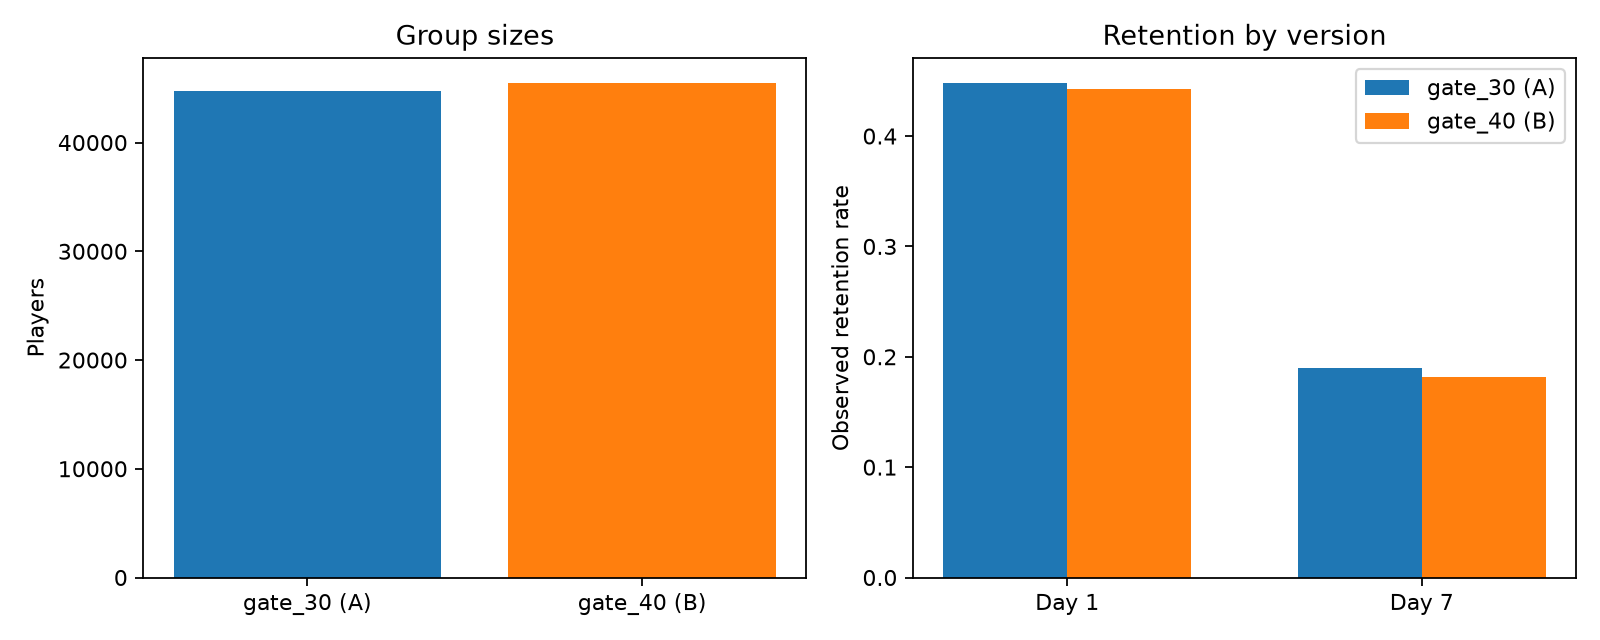
\includegraphics[width=0.9\textwidth]{real_data_group_sizes.png}
\caption{Left: players per version. Right: observed day-1 and day-7 retention by version.}
\end{figure}
\begin{figure}[H]
\centering
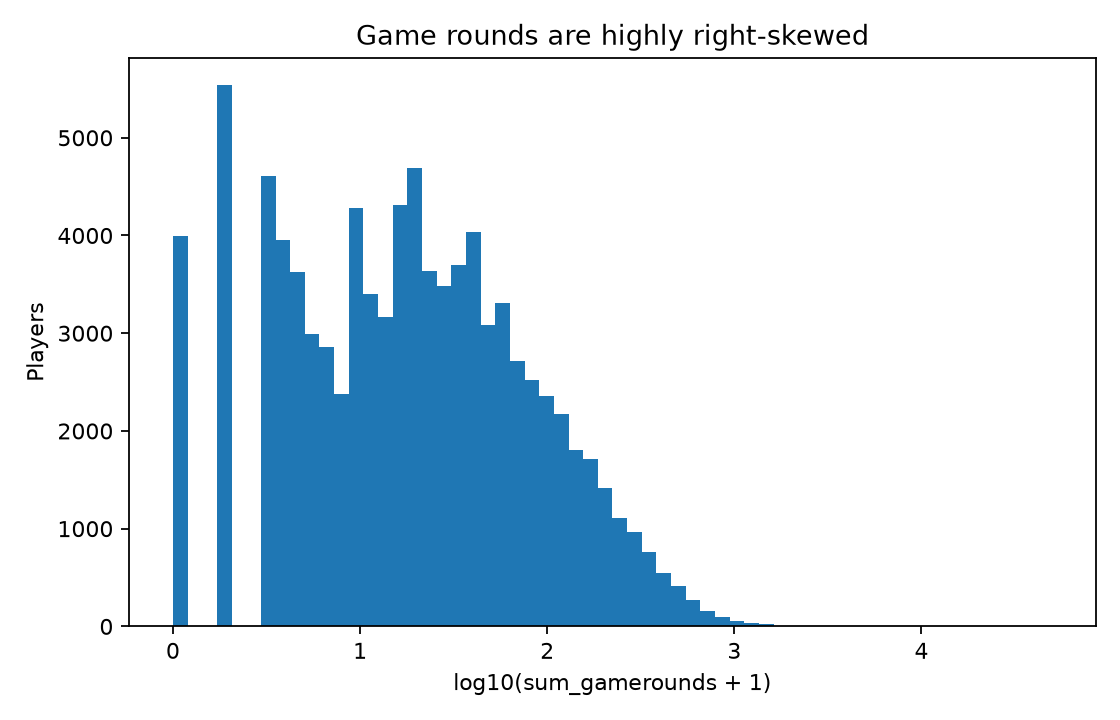
\includegraphics[width=0.6\textwidth]{real_data_gamerounds.png}
\caption{\texttt{sum\_gamerounds} is heavily right-skewed (log scale), with a few extreme players.}
\end{figure}

\subsection{Day-one retention (primary outcome)}
Group A has 20{,}034 returning players of 44{,}700 (44.8188\%); group B has 20{,}119 of 45{,}489 (44.2283\%). With independent $\Beta(1,1)$ priors the posteriors are $\Beta(20035,24667)$ and $\Beta(20120,25371)$, with 95\% credible intervals $[0.443582,0.452802]$ (A) and $[0.437724,0.446852]$ (B). With $M=200{,}000$ draws (seed 0), $\hat q=P(p_B>p_A\mid\text{data})=0.037055$ with $SE=0.000422$, and the 95\% interval for $p_B-p_A$ is $[-0.012376,\,0.000577]$. The pooled $z$-test gives $z=-1.784086$, two-sided $p=0.07440966$. The day-one difference is therefore not significant at 5\%, and the credible interval for the difference contains zero.

\subsection{Day-seven retention (secondary outcome)}
Group A has 8{,}502 of 44{,}700 (19.0201\%); group B has 8{,}279 of 45{,}489 (18.2000\%). Posteriors: $\Beta(8503,36199)$ and $\Beta(8280,37211)$, with 95\% intervals $[0.186590,0.193867]$ (A) and $[0.178482,0.185573]$ (B). With $M=200{,}000$, $\hat q=0.000805$ ($SE=0.000063$), and the 95\% interval for $p_B-p_A$ is $[-0.013263,\,-0.003113]$. The $z$-test gives $z=-3.164359$, $p=0.00155425$.
\begin{figure}[H]
\centering
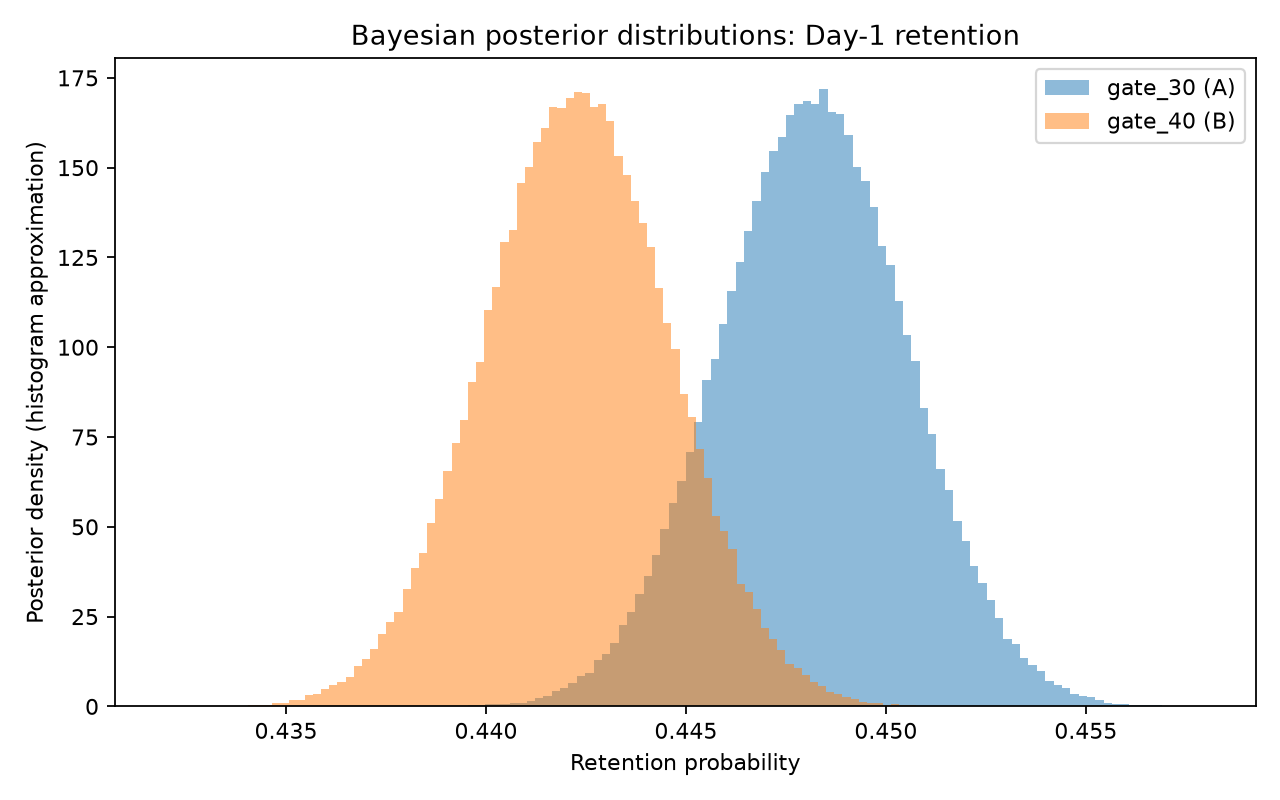
\includegraphics[width=0.48\textwidth]{real_data_retention_1_posterior.png}\hfill
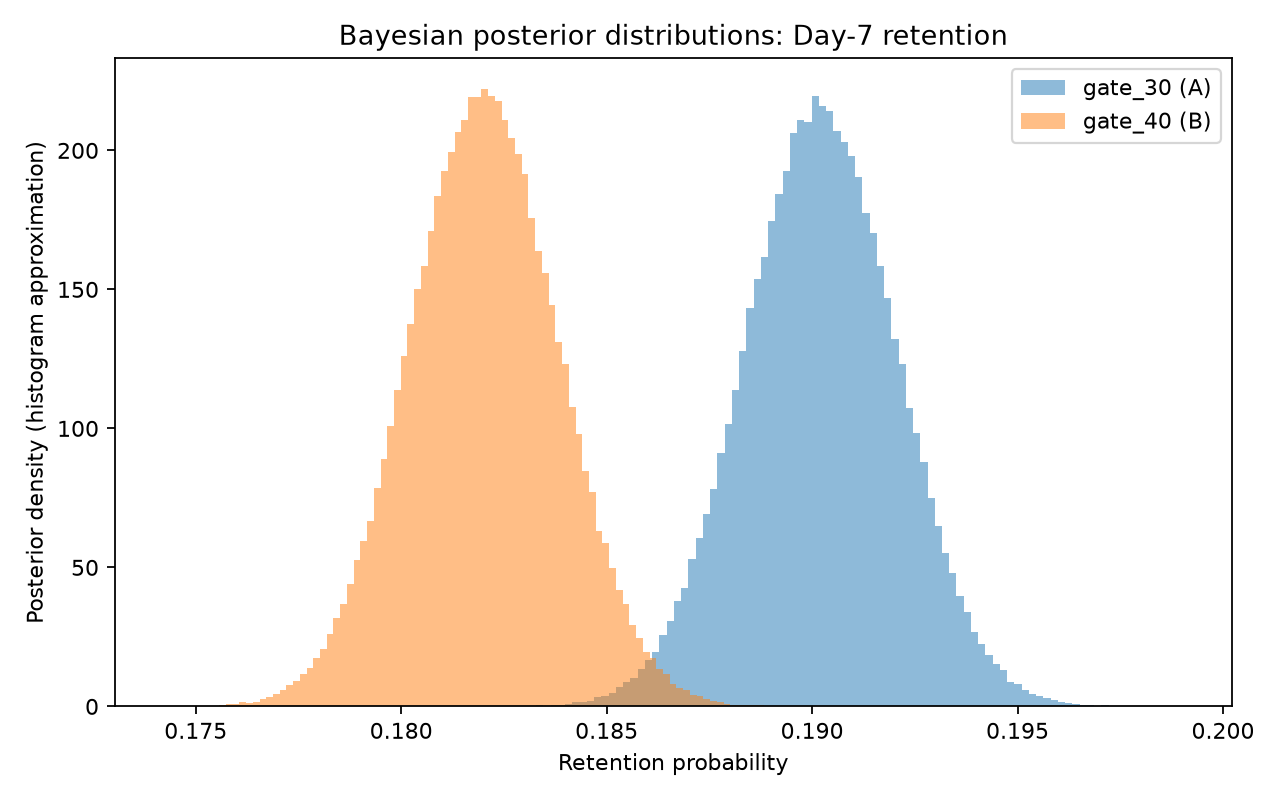
\includegraphics[width=0.48\textwidth]{real_data_retention_7_posterior.png}
\caption{Posterior distributions for day-1 (left) and day-7 (right) retention.}
\end{figure}
\begin{table}[H]
\centering
\caption{Bayesian and frequentist results (A $=$ \texttt{gate\_30}, B $=$ \texttt{gate\_40})}
\begin{tabular}{lrrrr}
\toprule
Outcome & A rate & B rate & $P(p_B>p_A\mid\text{data})$ & $z$-test $p$-value\\
\midrule
Day 1 & 44.8188\% & 44.2283\% & 3.7055\% & 0.07441\\
Day 7 & 19.0201\% & 18.2000\% & 0.0805\% & 0.00155\\
\bottomrule
\end{tabular}
\end{table}
Note that $P(p_B>p_A\mid\text{data})=0.037$ for day one is close to half the two-sided $p$-value $0.074$; this is expected with a flat prior and large $n$, but the two quantities answer different questions (posterior probability of a direction versus tail probability under $H_0$).

\section{Simulation check with known truth}
\label{sec:sim}
\textbf{Model.} True rates $p_A=0.10$, $p_B=0.12$; $n_A=n_B=1000$; $x_g\sim\mathrm{Binomial}(1000,p_g)$ drawn with \texttt{numpy.random.default\_rng(0)}; $\Beta(1,1)$ priors; $M=100{,}000$ posterior draws. Realized counts: $x_A=92$, $x_B=121$. The script is \texttt{src/simulation.py}.
\begin{table}[H]
\centering
\caption{True values versus estimates (seed 0)}
\begin{tabular}{lll}
\toprule
Quantity & True / reference value & Estimate\\
\midrule
$p_A$: posterior mean (95\% interval) & 0.1000 & 0.0928 $[0.0756,0.1115]$\\
$p_B$: posterior mean (95\% interval) & 0.1200 & 0.1218 $[0.1022,0.1427]$\\
Posterior variance of $p_A$ (formula vs.\ draws) & $8.395\times10^{-5}$ & $8.422\times10^{-5}$\\
Posterior variance of $p_B$ (formula vs.\ draws) & $1.0661\times10^{-4}$ & $1.0656\times10^{-4}$\\
$P(p_B>p_A\mid\text{data})$ (numerical integral vs.\ MC) & 0.98213 & 0.98189 ($SE$ 0.000422)\\
$z$ / two-sided $p$ (this sample) & -- & $2.102$ / $0.0355$\\
$z$-test Type-I error ($p_A=p_B=0.10$, 2000 reps) & 0.05 & 0.0425 (MC SE 0.0049)\\
$z$-test power ($p_A=0.10,p_B=0.12$, 2000 reps) & 0.2981 (theory) & 0.3210 (MC SE 0.0104)\\
\bottomrule
\end{tabular}
\end{table}
\begin{table}[H]
\centering
\caption{Monte Carlo standard error: 300 repetitions of $\hat q$ for each $M$}
\begin{tabular}{rrr}
\toprule
$M$ & Empirical SD of $\hat q$ & $\sqrt{q(1-q)/M}$\\
\midrule
100 & 0.01318 & 0.01325\\
1{,}000 & 0.00420 & 0.00419\\
10{,}000 & 0.00127 & 0.00133\\
\bottomrule
\end{tabular}
\end{table}
\textbf{What the simulation confirms, one derivation at a time.}
\begin{itemize}[nosep]
\item \emph{Q1--Q2 (likelihood, conjugacy):} both 95\% intervals from the $\Beta(1+x_g,\,1+n-x_g)$ posteriors contain the true rate, and the posterior means (0.0928, 0.1218) are close to 0.10 and 0.12.
\item \emph{Q3 (moments, weighted average):} the direct mean and the weighted average $(1-w)\mu_0+w\hat p$ agree to 10 decimals, and the formula-based and sample variance estimates closely agree.
\item \emph{Q4 (Monte Carlo):} $\hat q=0.98189$ is $0.57$ standard errors from the numerical-integral value $0.98213$, and the empirical SD of $\hat q$ follows $\sqrt{q(1-q)/M}$ across $M=100,1000,10000$ (Figure~\ref{fig:se}).
\item \emph{Q5 ($z$-test):} the Type-I error 0.0425 is within 1.5 Monte Carlo SEs of 0.05, and the simulated power 0.321 is within about 2.2 SEs of the large-sample power 0.298; the test is under-powered at $n=1000$ for a 2-point difference.
\end{itemize}
\begin{figure}[H]
\centering
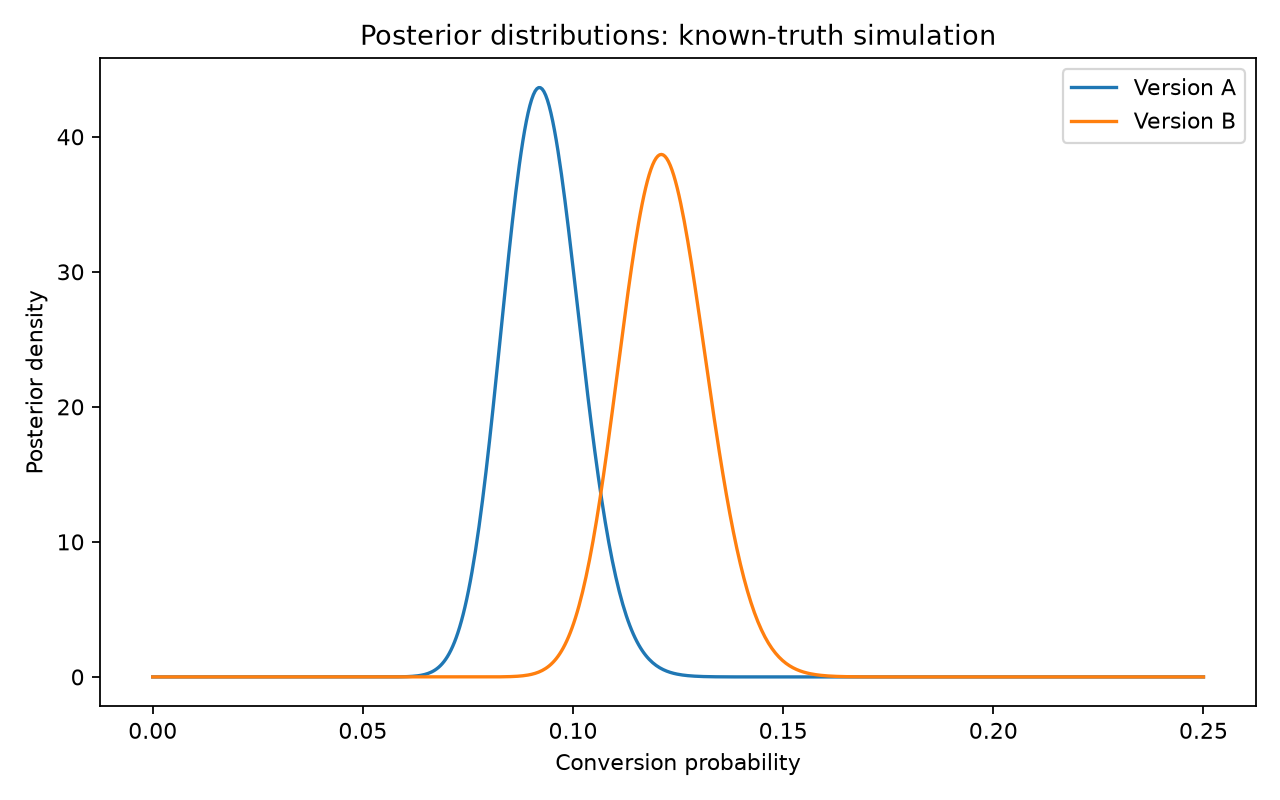
\includegraphics[width=0.48\textwidth]{simulation_posterior.png}\hfill
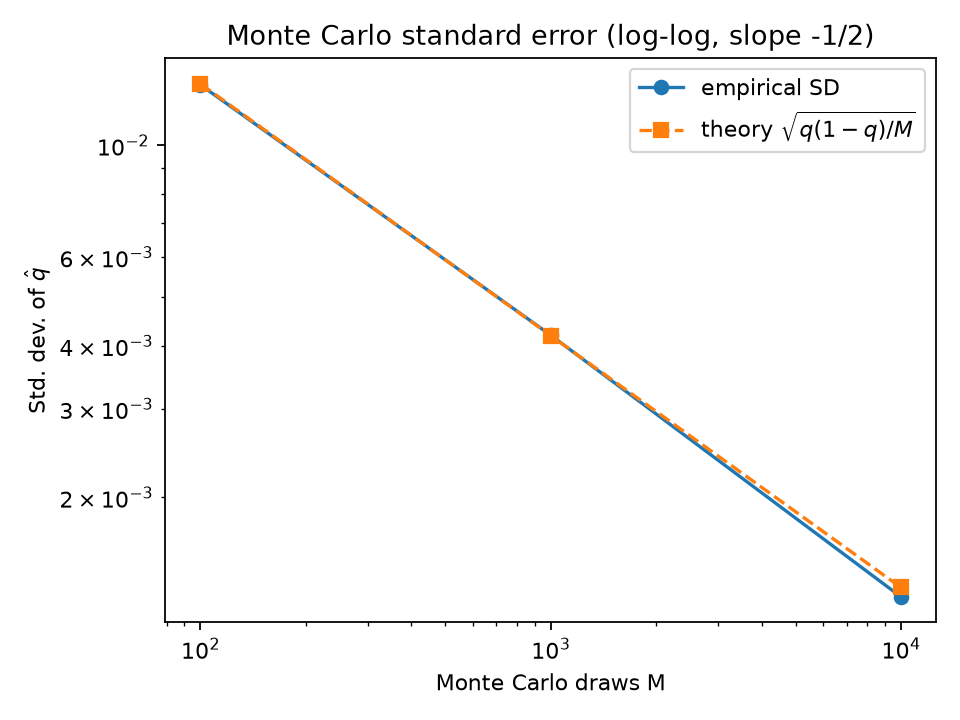
\includegraphics[width=0.48\textwidth]{simulation_mc_se_scaling.png}
\caption{Left: simulation posteriors. Right: Monte Carlo standard error versus $M$ (log--log).}\label{fig:se}
\end{figure}

\section{Team ownership and checking}
\textbf{Project Leader:} Kamya Kanara (assigns owners/checkers, maintains the task table in \texttt{docs/}, presents status at the check-in).
\begin{itemize}[nosep]
\item Rishita: Questions 1--3, notation and assumptions. Checker: Kamya Kanara.
\item Vaibhavi: Question 4, dataset description and simulation plots. Checker: Rishita.
\item Kamya Kanara: Question 5, code integration and numerical verification. Checker: Vaibhavi.
\end{itemize}
Each question above ends with its owner and checker; every member can explain every derivation.

\section{Conclusion}
The known-truth simulation agrees with the Beta--Binomial update, the posterior moments, the weighted-average identity, the Monte Carlo estimator and its standard error, and the pooled $z$-test. In Cookie Cats, \texttt{gate\_30} has a slightly higher day-one retention rate; the evidence is not conclusive at 5\% ($p=0.074$). For day seven, \texttt{gate\_30} is higher and both analyses give strong evidence ($P(p_B>p_A\mid\text{data})=0.08\%$, $p=0.0016$). These results describe retention in this dataset and do not explain why the groups differ. The group sizes are somewhat unbalanced ($p=0.0086$ for a 50/50 split), so Iteration 3 should examine assignment and logging, prior sensitivity and player subgroups. The Bayesian posterior probability and the frequentist $p$-value should not be interchanged.



\clearpage
\part*{Iteration 3: Implementation and Numerical Verification}
\addcontentsline{toc}{part}{Iteration 3: Implementation and Numerical Verification}

\section{Iteration 3 Overview}

Iteration 3 focuses on implementing the Bayesian A/B testing
methods developed in Iteration 2, verifying their numerical
accuracy, and evaluating their performance on simulated and
real-world data.

The main goal is to move beyond mathematical derivations
and demonstrate that our methods work correctly in practice.
We implement the core statistical calculations from scratch
using NumPy and compare our results with established SciPy
functions to check their accuracy.

This report begins with a small worked example to show
how Bayesian A/B testing works step by step. We calculate
posterior distributions, posterior means and variances,
the probability that one group performs better than the
other, and a frequentist two-proportion z-test.

Next, we use simulated data where the true conversion
probabilities are known. This allows us to measure
estimation errors, study how accuracy improves with
larger sample sizes, and verify our calculations against
independent numerical methods. We also examine a
stress-test scenario in which users appear in both
experimental groups, violating an important assumption.

Finally, we apply the same methods to the Cookie Cats
dataset, comparing 1-day and 7-day player retention
between the two experimental groups. We examine data
quality, verify the numerical results, and discuss
the assumptions and limitations of our analysis.

The report also includes the Iteration 3 mathematical
questions, numerical verification tables, simulation
results, an error convergence plot, team contributions
and independent checking, and a final discussion of
the findings.

\subsection{Implementation Files}

The implementation is organized into the following
Python files:

\begin{itemize}
    \item \texttt{src/methods.py}: Implements the core
    Bayesian and frequentist statistical methods.

    \item \texttt{src/small\_example.py}: Demonstrates
    the methods using a small numerical example.

    \item \texttt{src/simulate.py}: Generates synthetic
    A/B testing data with known probabilities.

    \item \texttt{src/check\_simulation.py}: Evaluates
    simulation accuracy, numerical verification,
    convergence, and stress tests.

    \item \texttt{src/run\_real.py}: Applies the methods
    to the Cookie Cats dataset and checks data quality
    and model assumptions.
\end{itemize}


% End here
\section{Iteration 3 -- Math Questions}
\subsection{Question 1: Posterior distributions, means, and variances}
For the new worked example, group A has $x_A=3$ clicks in $n_A=10$ visits, and group B has $x_B=5$ clicks in $n_B=10$ visits. We use independent uniform priors $p_A,p_B\sim\Beta(1,1)$. By Beta--Binomial conjugacy,
\begin{align*}
p_A\mid x_A,n_A&\sim\Beta(1+3,1+10-3)=\boxed{\Beta(4,8)},\\
p_B\mid x_B,n_B&\sim\Beta(1+5,1+10-5)=\boxed{\Beta(6,6)}.
\end{align*}
For $p\sim\Beta(\alpha,\beta)$,
\[
\E[p]=\frac{\alpha}{\alpha+\beta},\qquad
\Var(p)=\frac{\alpha\beta}{(\alpha+\beta)^2(\alpha+\beta+1)}.
\]
Consequently,
\begin{align*}
\E[p_A\mid\text{data}]&=\frac4{12}=\boxed{\frac13\approx0.333333},&
\Var(p_A\mid\text{data})&=\frac{4\cdot8}{12^2\cdot13}=\boxed{\frac{2}{117}\approx0.017094},\\
\E[p_B\mid\text{data}]&=\frac6{12}=\boxed{\frac12=0.500000},&
\Var(p_B\mid\text{data})&=\frac{6\cdot6}{12^2\cdot13}=\boxed{\frac1{52}\approx0.019231}.
\end{align*}
These exact fractions provide a hand-check of the posterior-moment implementation. The prior adds one pseudo-success and one pseudo-failure to each arm.

\subsection{Question 2: Monte Carlo estimate of $P(p_B>p_A\mid\mathrm{data})$}
Draw $M=100{,}000$ independent pairs $p_A^{(m)}\sim\Beta(4,8)$ and $p_B^{(m)}\sim\Beta(6,6)$. For $I_m=\mathbb{1}\{p_B^{(m)}>p_A^{(m)}\}$,
\[
\hat q=\frac1M\sum_{m=1}^M I_m,\qquad
\widehat{SE}_{MC}=\sqrt{\frac{\hat q(1-\hat q)}M}.
\]
The seeded run returned
\[
\boxed{\hat q=0.805370},\qquad
\boxed{\widehat{SE}_{MC}=0.001252}.
\]
Thus the posterior assigns approximately $80.5\%$ probability to B having the higher success probability. This is a posterior probability, not a frequentist $p$-value.

\subsection{Question 3: Two-proportion $z$-test and interpretation}
The observed rates are $\hat p_A=3/10=0.3$ and $\hat p_B=5/10=0.5$. Under $H_0:p_A=p_B$, the pooled rate is
\[
\hat p_{\mathrm{pool}}=\frac{3+5}{10+10}=0.4.
\]
The standard error under the null and test statistic are
\begin{align*}
SE_0&=\sqrt{0.4(0.6)\left(\frac1{10}+\frac1{10}\right)}=\sqrt{0.048}\approx0.219089,\\
z&=\frac{0.5-0.3}{\sqrt{0.048}}=\boxed{0.912871}.
\end{align*}
The two-sided normal-approximation $p$-value is
\[
\boxed{p_{\mathrm{two\text{-}sided}}=2\bigl[1-\Phi(|z|)\bigr]\approx0.361310}.
\]
At $\alpha=0.05$ we do not reject equality of the proportions. This does not contradict the Bayesian $P(p_B>p_A\mid\text{data})\approx0.805$: the methods answer different questions. Because the example has only ten visits per arm, the normal approximation is also relatively rough; the assignment nevertheless requests this $z$-test.

\subsection{Question 4: Independent grid integration}
With independent posteriors, the exact target probability can be written as
\[
q=P(p_B>p_A\mid\text{data})
=\int_0^1 f_B(y)\left[\int_0^y f_A(x)\,dx\right]dy
=\int_0^1 f_B(y)F_A(y)\,dy.
\]
Our \texttt{my\_grid\_probability} evaluates Beta densities on a uniform grid and uses cumulative trapezoidal integration for $F_A$ followed by trapezoidal integration of $f_BF_A$. With 10,001 grid points, the result is $0.8065015429$. Independently, SciPy's adaptive quadrature gives $0.8065015480$:
\begin{table}[H]\centering
\caption{Small-example probability verification.}
\begin{tabular}{lr}\toprule
Method & $P(p_B>p_A\mid\mathrm{data})$\\\midrule
Custom grid & 0.8065015429\\
SciPy adaptive quadrature & 0.8065015480\\
Monte Carlo ($M=100{,}000$) & 0.8053700000\\
Absolute grid--quadrature difference & $5.04\times10^{-9}$\\
Monte Carlo SE & 0.001252\\
Monte Carlo discrepancy / SE & 0.904\\\bottomrule
\end{tabular}
\end{table}
The grid--quadrature error is below $10^{-6}$; the Monte Carlo result is within three estimated standard errors of the quadrature result.

\subsection{Question 5: Cookie Cats real-data analysis and data checks}
The real dataset is \texttt{data/cookie\_cats.csv}. We define A as \texttt{gate\_30} and B as \texttt{gate\_40}. Each \texttt{userid} is checked for duplicate rows and membership in more than one group; both counts are zero. There are no missing values in the required fields, and both retention columns contain binary outcomes.
\begin{table}[H]\centering
\caption{Real-data integrity and allocation.}
\begin{tabular}{lr}\toprule
Check & Result\\\midrule
Total observations & 90,189\\
Group A: \texttt{gate\_30} & 44,700\\
Group B: \texttt{gate\_40} & 45,489\\
A/B group-size ratio & 0.9827\\
Duplicate user IDs & 0\\
Users appearing in both groups & 0\\
Missing required values & 0\\\bottomrule
\end{tabular}
\end{table}
The assignment's Bayesian, Monte Carlo, credible-interval, and two-proportion $z$-test methods were applied separately to day-one and day-seven retention.
\begin{table}[H]\centering\small
\caption{Iteration 3 Cookie Cats results (B minus A).}
\begin{tabular}{lrr}\toprule
Quantity & Day 1 & Day 7\\\midrule
A retained / total & 20,034 / 44,700 & 8,502 / 44,700\\
B retained / total & 20,119 / 45,489 & 8,279 / 45,489\\
Observed rate A & 0.448188 & 0.190201\\
Observed rate B & 0.442283 & 0.182000\\
Posterior mean A & 0.448190 & 0.190215\\
Posterior mean B & 0.442285 & 0.182014\\
Posterior variance A & 0.00000553 & 0.00000345\\
Posterior variance B & 0.00000542 & 0.00000327\\
MC $P(p_B>p_A\mid\mathrm{data})$ & 0.037000 & 0.000890\\
MC standard error & 0.000597 & 0.000094\\
95\% credible interval for $p_B-p_A$ & $[-0.012376,\ 0.000577]$ & $[-0.013288,\ -0.003113]$\\
Two-proportion $z$ & $-1.784086$ & $-3.164359$\\
Two-sided $p$-value & 0.074410 & 0.001554\\\bottomrule
\end{tabular}
\end{table}
For day one, the two-sided $p$-value exceeds 0.05 and the credible interval for B--A crosses zero. For day seven, the $p$-value is below 0.05 and the interval is entirely negative, favoring A (\texttt{gate\_30}). The observed differences are associations within the randomized experiment and do not by themselves identify a mechanism.

\section{Implementation and independent numerical verification}
\subsection{From-scratch methods and library comparisons}
The custom posterior update computes $(\alpha,\beta)=(a+x,b+n-x)$, and the custom posterior-moment function evaluates the closed-form mean and variance. The Monte Carlo routine samples independent Beta posteriors, estimates the fraction of draws with $p_B>p_A$, and reports the Bernoulli Monte Carlo SE. The grid routine uses NumPy-based numerical integration; the $z$-test computes the pooled null standard error and two-sided normal-tail probability. A separate function draws posterior samples to estimate a 95\% credible interval for $p_B-p_A$. SciPy is not used to implement these core routines.

\begin{table}[H]\centering\small
\caption{Independent checks on the real-data posterior and probability calculations.}
\begin{tabular}{llrr}\toprule
Outcome & Quantity & Custom result & SciPy result\\\midrule
Day 1 & Mean A & 0.44819024 & 0.44819024\\
Day 1 & Mean B & 0.44228529 & 0.44228529\\
Day 1 & $P(p_B>p_A)$ (MC vs quad) & 0.037000 & 0.037206\\
Day 7 & Mean A & 0.19021520 & 0.19021520\\
Day 7 & Mean B & 0.18201402 & 0.18201402\\
Day 7 & $P(p_B>p_A)$ (MC vs quad) & 0.000890 & 0.000777\\\bottomrule
\end{tabular}
\end{table}
The reported absolute errors for all four real-data posterior means and variances versus SciPy were zero at the printed precision. The Monte Carlo--quadrature discrepancies were $0.345$ SE (day one) and $1.195$ SE (day seven), both within three SE. These Monte Carlo discrepancies are sampling error, not machine-precision agreement.

\subsection{Simulation with known truth}
The Iteration 3 simulation retains the Iteration 2 model and settings: $p_A=0.10$, $p_B=0.12$, $n_A=n_B=1000$, and seed 0. The current generator draws the two Bernoulli outcome vectors with NumPy and obtains $x_A=96$ and $x_B=118$. Therefore,
\[
\begin{array}{ll}
\E[p_A\mid\mathrm{data}]=97/1002=0.09680639,&
\E[p_B\mid\mathrm{data}]=119/1002=0.11876248,\\
|\E[p_A\mid\mathrm{data}]-0.10|=0.003194,&
|\E[p_B\mid\mathrm{data}]-0.12|=0.001238.
\end{array}
\]
The current simulation's Monte Carlo estimate is $P(p_B>p_A\mid\mathrm{data})\approx0.943500$, with SE $0.000730$. The posterior means and variances agree with SciPy's \texttt{beta.mean} and \texttt{beta.var} at printed precision.

\textbf{Reproducibility note.} The retained Iteration 2 report records $x_A=92$ and $x_B=121$ for its simulation, while the current Iteration 3 script produces 96 and 118. The model, parameter values, sample sizes, and nominal seed are unchanged, but the sample realizations differ. This can occur when the random-number generator or its sequence of calls differs; the exact historical cause has not been independently established. Accordingly, the two iterations' simulated posterior values should not be compared as if they were computed from the same realized dataset.

\subsection{Grid, quadrature, and Monte Carlo verification on simulation}
For the current simulated posteriors, the independent comparison is
\begin{table}[H]\centering
\caption{Known-truth simulation probability verification.}
\begin{tabular}{lr}\toprule
Method or diagnostic & Result\\\midrule
Custom grid ($10{,}001$ points) & 0.9439498682\\
SciPy adaptive quadrature & 0.9439506518\\
Custom Monte Carlo ($100{,}000$ draws) & 0.9435000000\\
Monte Carlo SE & 0.0007301216\\
Grid absolute error & $7.84\times10^{-7}$\\
Monte Carlo discrepancy / SE & 0.617\\\bottomrule
\end{tabular}
\end{table}
The grid error is less than the specified $10^{-6}$ tolerance, and the Monte Carlo estimate lies within three SE of both the grid and SciPy quadrature values. The grid result passes the stated tolerance but is closer to the threshold than in the small example.

\subsection{Sample-size scaling and error-convergence plot}
The simulation was run at multiple sample sizes. The single-realization posterior-mean absolute errors and the RMSE over 200 replications are distinct diagnostics; the latter is more stable for assessing convergence.
\begin{table}[H]\centering\small
\caption{Error convergence over 200 independent repetitions per sample size.}
\begin{tabular}{rrr}\toprule
$n$ per group & RMSE of A posterior mean & RMSE of B posterior mean\\\midrule
100 & 0.028575 & 0.033105\\
300 & 0.016789 & 0.018140\\
1,000 & 0.009488 & 0.009910\\
3,000 & 0.005472 & 0.005648\\
10,000 & 0.002887 & 0.003088\\\bottomrule
\end{tabular}
\end{table}
Both errors generally decrease with sample size, consistent with the $O(n^{-1/2})$ scale of binomial sampling uncertainty. The log--log plot was generated by \texttt{src/check\_simulation.py} and saved as \texttt{src/error\_convergence.png}.
\begin{figure}[H]\centering
\IfFileExists{figures/error_convergence.png}{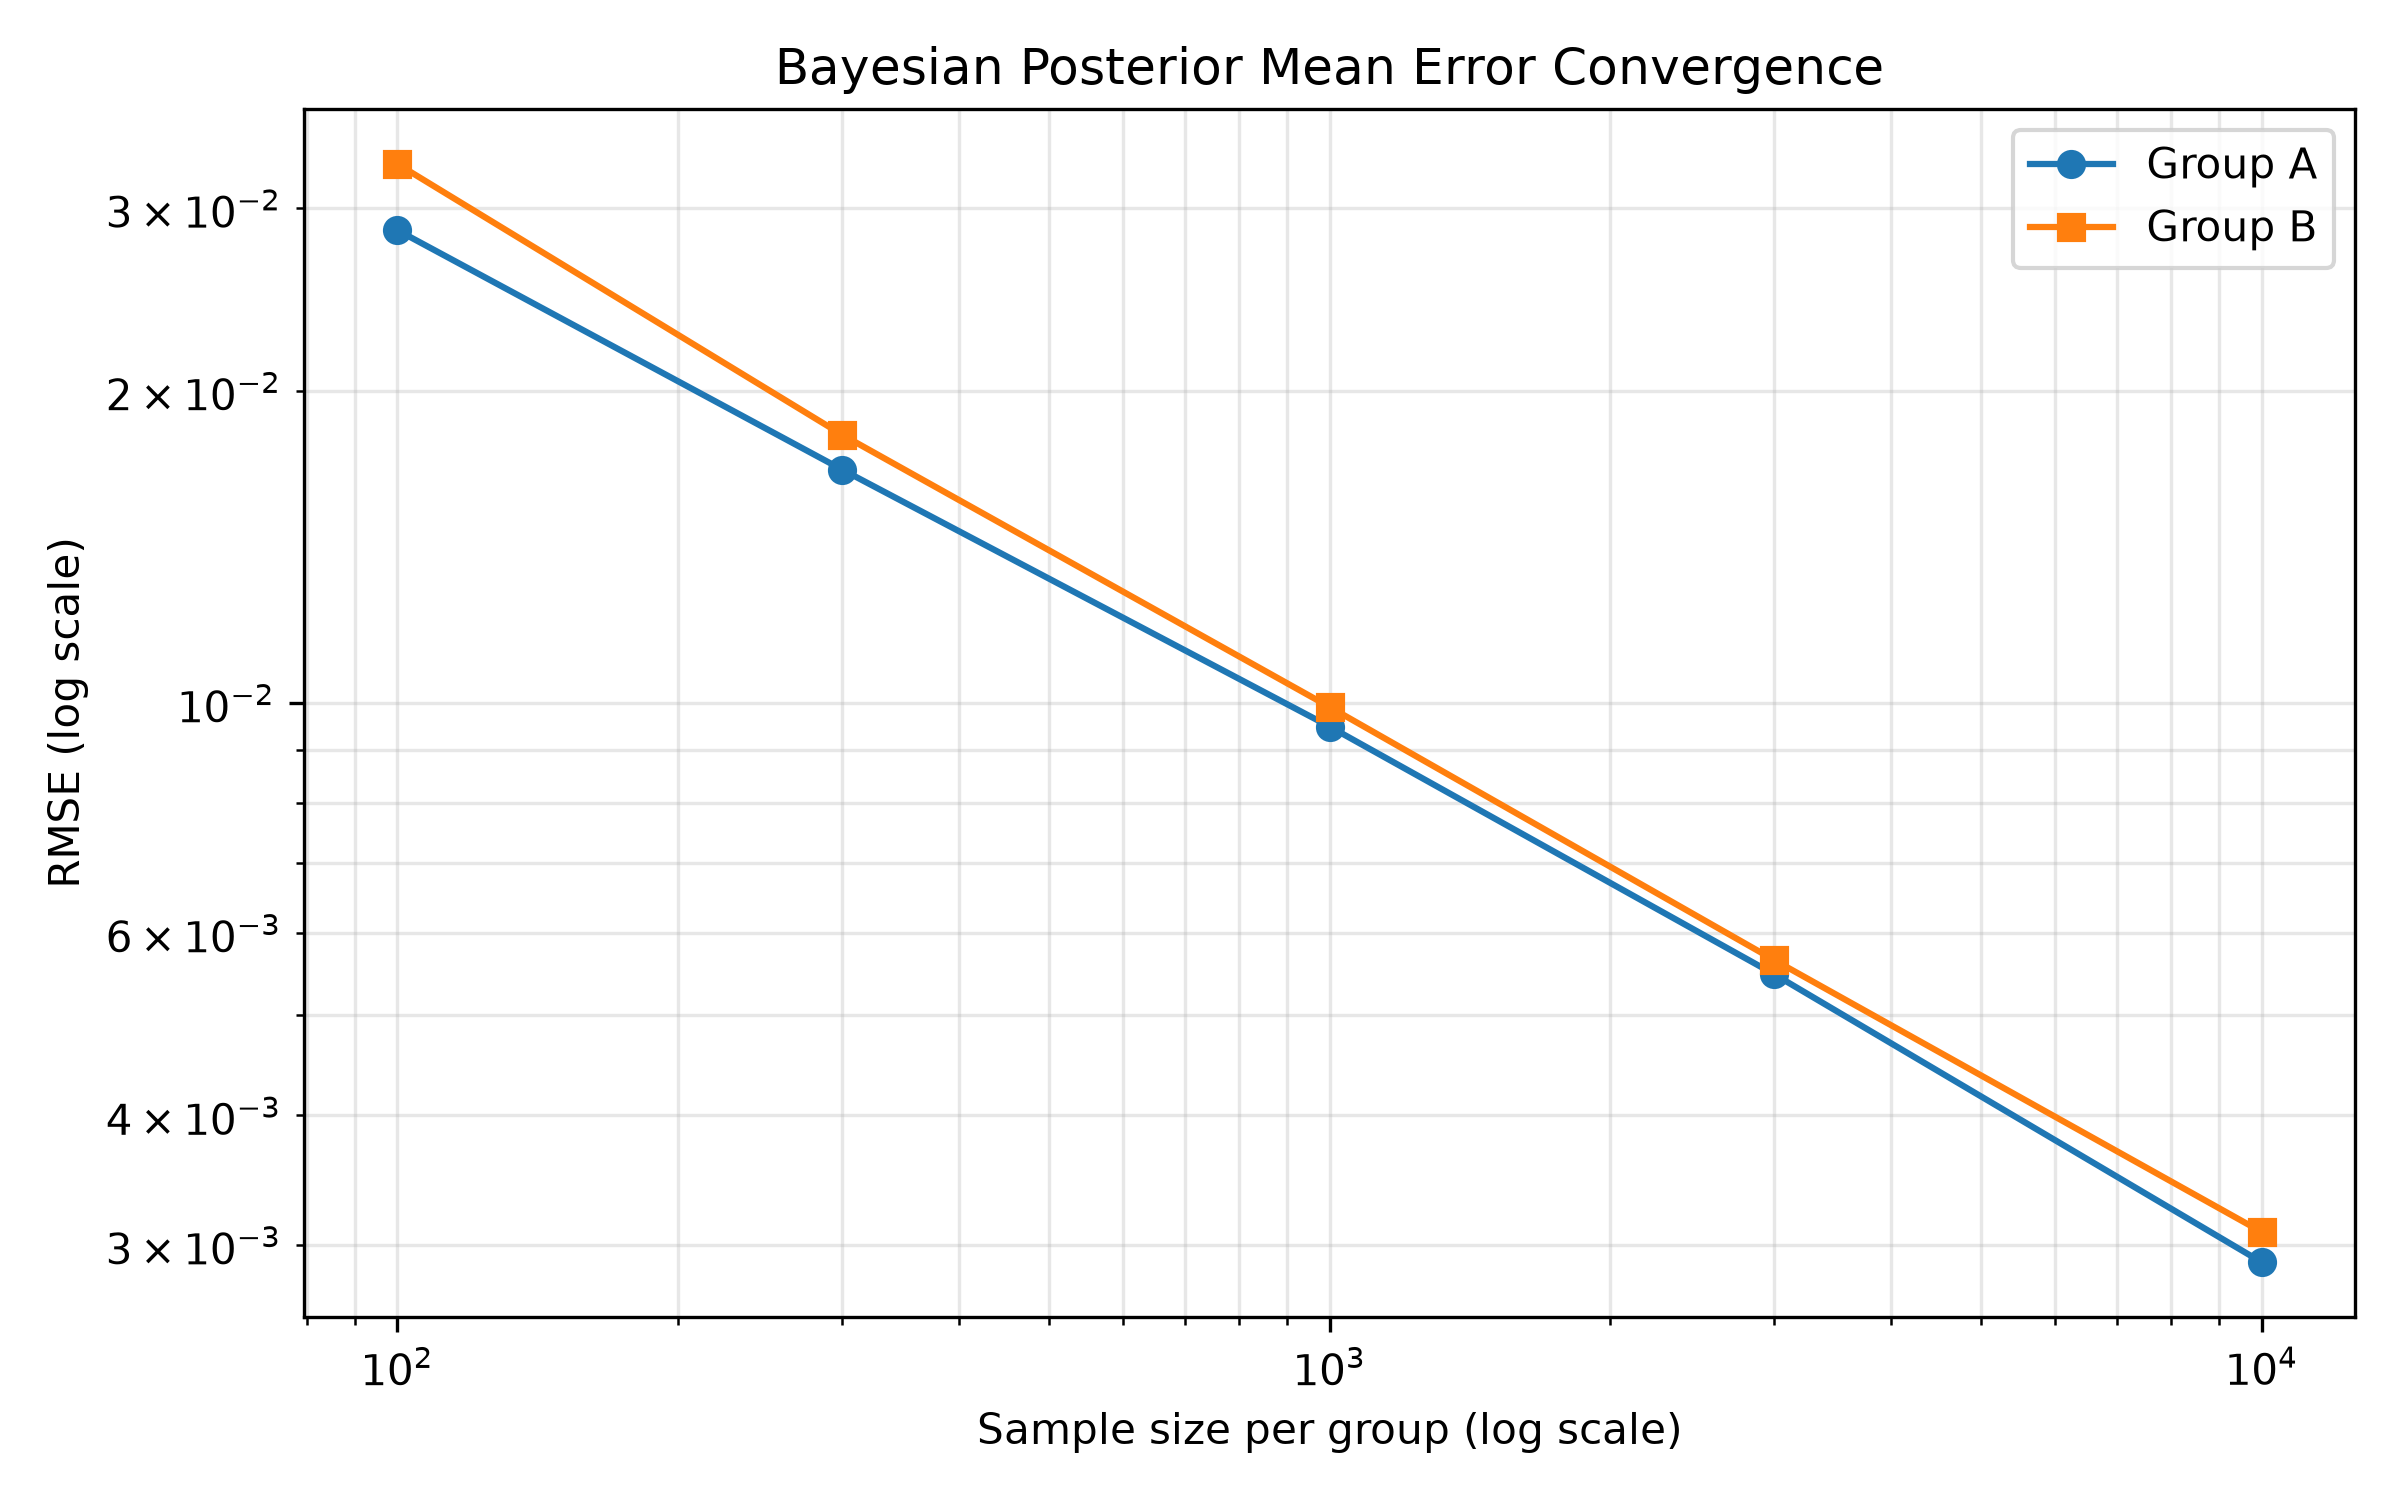
\includegraphics[width=0.82\textwidth]{figures/error_convergence.png}}{\fbox{\parbox{0.8\textwidth}{\centering Upload \texttt{src/error\_convergence.png} to Overleaf as \texttt{figures/error\_convergence.png}.}}}
\caption{Iteration 3 log--log error-convergence experiment (200 replications per sample size).}\label{fig:iter3convergence}
\end{figure}

\subsection{Null rejection-frequency check}
To verify the frequentist test under the null, we generated 1,000 experiments with $p_A=p_B=0.10$, $n_A=n_B=1000$, and a fixed generator seed of 0. We rejected $H_0$ when the two-sided $p$-value was below 0.05. There were 49 rejections:
\[
\widehat{P}(\mathrm{reject}\mid H_0)=\frac{49}{1000}=\boxed{0.049=4.9\%}.
\]
The result is within the assignment's $5\%\pm1.4\%$ acceptance range ($3.6\%$ to $6.4\%$). It is an empirical calibration check, not proof that the test is valid under every data-generating process.

\subsection{Stress tests and overlapping users}
The implementation also tested zero successes in both arms, all successes in both arms, and extreme arm differences; posterior calculations remained finite, with approximately 0.5 posterior superiority probability for the symmetric cases and approximately 1.0 for the extreme difference.

The required assumption-violation test assigned 1,000 records to each arm but deliberately reused 100 user IDs across both arms, yielding 10\% overlap relative to each arm. The duplicate-assignment check correctly failed. If the two arms are nevertheless treated as independent, the resulting naive two-proportion test reported $z=1.591439$ and two-sided $p=0.111511$.

\textbf{Interpretation and limitation.} The overlap invalidates the clean disjoint-group assignment design. In the current stress-test code, outcomes for the reused IDs are generated independently in each arm; therefore, the example establishes a user-assignment violation but does \emph{not} measure a covariance-induced bias or change in the true sampling variance. With correlated repeated-user outcomes, an independent-arm standard error may be miscalibrated. The correct remedy depends on the experiment design: prevent cross-arm assignment, or use an analysis that explicitly models repeated/paired observations.

\section{Assumption checks and limitations}
\begin{itemize}[nosep]
\item \textbf{Simulation:} Positive group sizes, valid binary success counts, and positive Beta prior parameters passed. Independent Bernoulli outcomes and fixed probabilities are specified by the simulation generator; random assignment of a shared user pool is not explicitly modeled in the baseline simulation.
\item \textbf{Real data:} All 90,189 rows had the required fields; user IDs were unique, no users appeared in both groups, and day-one/day-seven outcomes were binary. Group sizes were 44,700 and 45,489 (A/B ratio 0.9827).
\item \textbf{Not directly verifiable from the CSV:} independence between distinct users, actual randomization procedures, stable within-arm success probabilities, and absence of unrecorded repeated exposure. The group-size imbalance noted in Iteration 2 remains a design/logging question, not proof of a particular failure.
\item \textbf{Inference:} The uniform $\Beta(1,1)$ prior is a modeling choice. Day-one and day-seven outcomes are analyzed separately; they are measured on the same users and should not be interpreted as independent experiments.
\end{itemize}

\section{Reproducibility and deliverables}
Run the following commands from the repository root after installing NumPy, pandas, SciPy, and Matplotlib:
\begin{verbatim}
python src/small_example.py
python src/check_simulation.py
python src/run_real.py
\end{verbatim}
The code and the convergence image are on GitHub branch \texttt{iteration3}, commit \texttt{530a4e1}. The convergence image must also be uploaded to the Overleaf \texttt{figures/} folder for inclusion in the compiled PDF. The repository README should list the commands above and the Python dependencies. Each student should submit the required GitHub and read-only Overleaf links as instructed in the assignment.

\section{Iteration 3 team leadership, ownership, and checking}
\textbf{Project leader: Rishita Chawla.} Leadership rotated from Kamya Kanara in Iteration 2 to Rishita Chawla in Iteration 3. The leader coordinates progress, makes sure the numerical checks and report are complete, and helps the team prepare its final submission. Leadership is separate from individual ownership of each mathematical derivation or code component.

The assignment requires each team member to own mathematics and code and to have another team member independently check the work. The final owner--checker assignments must match the team's updated Excel project plan. They have not been confirmed in the material available for this report, so the table below is a completion checklist rather than a claim that specific members performed the checks.

\begin{table}[H]
\centering
\small
\begin{tabular}{p{0.48\textwidth}p{0.18\textwidth}p{0.18\textwidth}}
\toprule
\textbf{Iteration 3 work} & \textbf{Owner} & \textbf{Independent checker}\\
\midrule
Worked example and mathematical answers & Rishita &  Kamya\\
Core Bayesian and frequentist methods & Kamya & Vaibhavi\\
Simulation, convergence, and stress tests & Rishita & Vaibhavi\\
Cookie Cats analysis and numerical verification & Rishita & Vaibhavi\\
Overleaf report and reproducibility review & Vaibhavi & Rishita\\
\bottomrule
\end{tabular}
\caption{Iteration 3 task ownership and checking}
\end{table}


\section{Iteration 3 conclusion}
The from-scratch Beta posterior, posterior moments, Monte Carlo probability, grid integration, credible interval, and two-proportion $z$-test were applied to a small example, known-truth simulation, and real Cookie Cats retention data. The small-example grid agreed with adaptive quadrature within $5.04\times10^{-9}$, and the known-truth simulation grid agreed within $7.84\times10^{-7}$; both satisfy the $10^{-6}$ criterion. Monte Carlo results were within three estimated standard errors of the independent numerical reference. Under 1,000 null simulations, the $z$-test rejected 4.9\% of the time, inside the required acceptance range. A 10\% overlapping-user stress test correctly exposed an assignment-design violation. On Cookie Cats, the day-one difference was not significant in the two-sided $z$-test, whereas day-seven retention favored \texttt{gate\_30}. These findings validate the reported numerical implementation under the tested conditions while retaining the design and modeling caveats above.

\nocite{*}
\bibliographystyle{plain}
\bibliography{references}
\end{document}
